\documentclass[tikz,border=10pt]{standalone}
\usepackage{xcolor}
\usepackage{amsmath} % Bổ sung gói này để sử dụng lệnh \text{}
\usetikzlibrary{positioning, arrows.meta, calc}

% Định nghĩa bảng màu
\definecolor{boxbg}{HTML}{EBF3FA}      % Xanh nhạt làm nền khối
\definecolor{boxborder}{HTML}{2C3E50}  % Xanh đen làm viền khối
\definecolor{arrowcolor}{HTML}{34495E} % Màu đường mũi tên
\definecolor{labelgray}{HTML}{555555}  % Màu chữ ghi chú

\begin{document}
	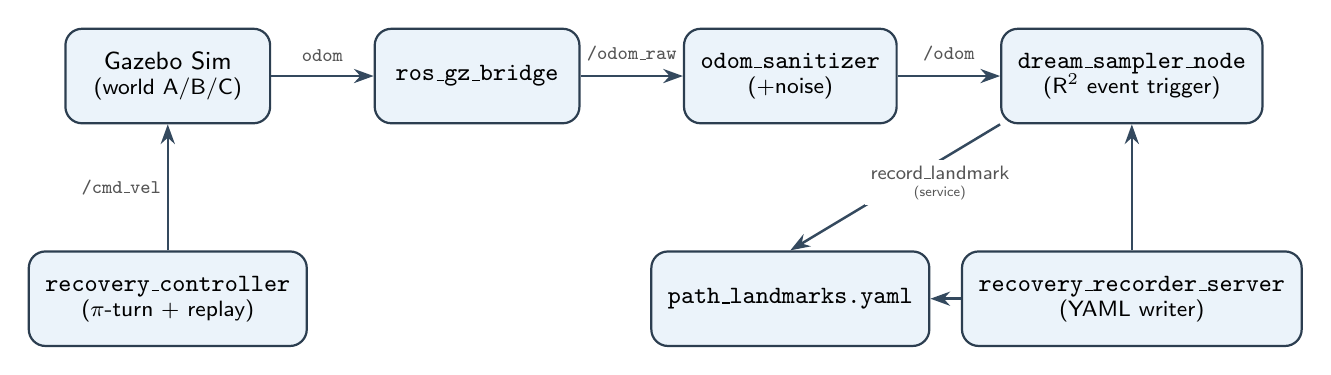
\begin{tikzpicture}[
		block/.style={
			draw=boxborder,
			fill=boxbg,
			rounded corners=6pt,
			line width=0.8pt,
			minimum height=1.2cm,
			minimum width=2.6cm,
			align=center,
			font=\sffamily\small,
			inner sep=6pt
		},
		arrow/.style={
			-{Stealth[length=2.5mm, width=1.8mm]},
			line width=0.9pt,
			draw=arrowcolor
		},
		lbl/.style={
			font=\sffamily\scriptsize,
			text=labelgray,
			fill=white,
			inner sep=2pt,
			align=center
		}
		]
		
		% --- HÀNG 1: LUỒNG XỬ LÝ CHÍNH ---
		\node[block] (gazebo) {Gazebo Sim\\[-2pt]\footnotesize(world A/B/C)};
		
		\node[block, right=1.3cm of gazebo] (bridge) {\texttt{ros\_gz\_bridge}};
		
		\node[block, right=1.3cm of bridge] (sanitizer) {\texttt{odom\_sanitizer}\\[-2pt]\footnotesize(+noise)};
		
		\node[block, right=1.3cm of sanitizer] (dream) {\texttt{dream\_sampler\_node}\\[-2pt]\footnotesize($\text{R}^2$ event trigger)};
		
		% --- HÀNG 2: CÁC KHỐI ĐIỀU KHIỂN & LƯU TRỮ ---
		\node[block, below=1.6cm of gazebo] (controller) {\texttt{recovery\_controller}\\[-2pt]\footnotesize($\pi$-turn + replay)};
		
		\node[block, below=1.6cm of sanitizer] (landmarks) {\texttt{path\_landmarks.yaml}};
		
		\node[block, below=1.6cm of dream] (recorder) {\texttt{recovery\_recorder\_server}\\[-2pt]\footnotesize(YAML writer)};
		
		% --- ĐƯỜNG NỐI & NHÃN CHỮ ---
		\draw[arrow] (gazebo) -- node[lbl, above=0.1cm] {\texttt{odom}} (bridge);
		\draw[arrow] (bridge) -- node[lbl, above=0.1cm] {\texttt{/odom\_raw}} (sanitizer);
		\draw[arrow] (sanitizer) -- node[lbl, above=0.1cm] {\texttt{/odom}} (dream);
		
		\draw[arrow] (controller) -- node[lbl, left] {\texttt{/cmd\_vel}} (gazebo);
		
		\draw[arrow] (dream.south west) -- node[lbl, above right, pos=0.65] {record\_landmark\\[-2pt]\tiny(service)} (landmarks.north);
		
		\draw[arrow] (recorder) -- (landmarks);
		
		\draw[arrow] (recorder) -- (dream);
		
	\end{tikzpicture}
\end{document}